%%
%% KCGS journal latex format example.
%% There are several options in this file, 
%% PLEASE READ THE FOLLOWING LINES BEFORE YOU USE.
%% 1. If you use KC2007 instead of MikTeX, use ``kotex'' package.
%% 2. If you don't have ``ifpdf'' package, 
%%    then use ``epsfig'' and ``epstopdf'' packages.
%%    (But usually you should have ``ifpdf'' package, 
%%    because the package is used in siggraph class.
%% 3. If you don't have ``caption'' package, 
%%    comment out "\usepackage[labelfont=bf]{caption}" command.
%% 4. There are several commands for squeezing figures and tables into a page.
%%    Uncomment those commands if you want to use them.
%% This file is tested under KC2008 and MikTex 2.4~2.5 with HLaTeX.
%%
%% If you have problems in using LaTeX, visit http://www.ktug.or.kr
%%
%% - 1st version 2007/08/22 Hyunjun Lee.
%% - 2nd version 2009/03/11 Hyunjun Lee.
%%   email: crowlove@postech.ac.kr
%%   Please do not email me if you have any questions or problems :)
%%

\documentclass[a4paper,twocolumn]{article}

%---------------------------------------------------------------------------
%% If you don't really know latex commands and changes you want to make,
%% you don't need to change anything up to "document begins" below.

\usepackage[hangul]{kotex}
\usepackage{dhucs-cmap}

%% Geometry package for page layout.
\usepackage{geometry}
\geometry{width=190mm, height=247mm, hmargin={1cm, 1cm}, vmargin={3cm, 2cm}}

%% We use one-half spacing.
\usepackage{setspace}
\onehalfspacing

%% Package to use both korean and english titles, authors, abstracts.
\usepackage{kcgs_utf}

%% The 'helvet' and 'times' packages define the typefaces used for
%% serif and sans serif type in this document. Computer Modern Roman 
%% is used for mathematics typesetting. The scale factor is set to .92
%% to bring the sans-serif type in line with the serif type.
\usepackage[scaled=.92]{helvet}
\usepackage{times}

%% The 'graphicx' package allows for the inclusion of EPS figures.
\usepackage{ifpdf}
	\ifpdf % compile with pdflatex
		\usepackage[pdftex]{graphicx}
	\else % latex => compile with dvipdfmx
		\usepackage{graphicx}
			\DeclareGraphicsExtensions{.jpg,.pdf,.png,.eps}
			\DeclareGraphicsRule{.jpg}{eps}{.bb}{}
			\DeclareGraphicsRule{.pdf}{eps}{.bb}{}
			\DeclareGraphicsRule{.png}{eps}{.bb}{}
	\fi

%% Or, if you don't have ``ifpdf'' package, use this two packages instead.
%\usepackage{epsfig}
%\usepackage{epstopdf}

%% Remove '제','절' from section names.
\kscntformat{section}{}{.}

%% Optional: the 'caption' package provides a nicer-looking replacement
%% for the standard caption environment. With 'labelfont=bf,'textfont=it',
%% caption labels are bold and caption text is italic.
%% You don't have to use this package if the package does not exist.
%\usepackage[labelfont=bf]{caption}

%% Uncomment following lines if you want to squeeze figures and tables into a page.
%\renewcommand{\topfraction}{0.95}
%\setcounter{bottomnumber}{1}
%\renewcommand{\bottomfraction}{0.95}
%\setcounter{totalnumber}{3}
%\renewcommand{\textfraction}{0.05}
%\renewcommand{\floatpagefraction}{0.95}
%\setcounter{dbltopnumber}{2}
%\renewcommand{\dbltopfraction}{0.95}
%\renewcommand{\dblfloatpagefraction}{0.95}

%---------------------------------------------------------------------------
% document begins

\begin{document}

%% Title.
\title{Sparse Ellipsometry: Portable Acquisition of Polarimetric SVBRDF	and Shape with Unstructured Flash Photography}

%% Author names.
\author{황인승$^{1\circ}$
\and 전석준$^{1}$
\and Adolfo Muñoz$^{3}$
\and Diego Gutierrez$^{3}$
\and Xin Tong$^{2}$
\and 김민혁$^{1*}$}

\affiliation{$^{1}$KAIST 
	\hspace{5mm} $^{2}$Microsoft Research Asia 
	\hspace{5mm} $^{3}$Universidad de Zaragoza - I3A}

\authoremail{
	$^{1}$\{ishwang, sjjeon, minhkim\}@vclab.kaist.ac.kr \hspace{5mm}
	$^{2}$xtong@microsoft.com \hspace{5mm}
	$^{3}$\{adolfo, didgog\}@unizar.es}

%% English title.
\entitle{Sparse Ellipsometry: Portable Acquisition of Polarimetric SVBRDF	and Shape with Unstructured Flash Photography}

%% English author names.
\enauthor{Inseung Hwang$^{1\circ}$
	\and Daniel S. Jeon$^{1}$
	\and Adolfo Muñoz$^{3}$
	\and Diego Gutierrez$^{3}$
	\and Xin Tong$^{2}$
	\and Min H. Kim$^{1*}$}

\enaffiliation{$^{1}$KAIST 
	\hspace{5mm} $^{2}$Microsoft Research Asia 
	\hspace{5mm} $^{3}$Universidad de Zaragoza - I3A}

%% (Optional) Teaser
%\teaser{
%  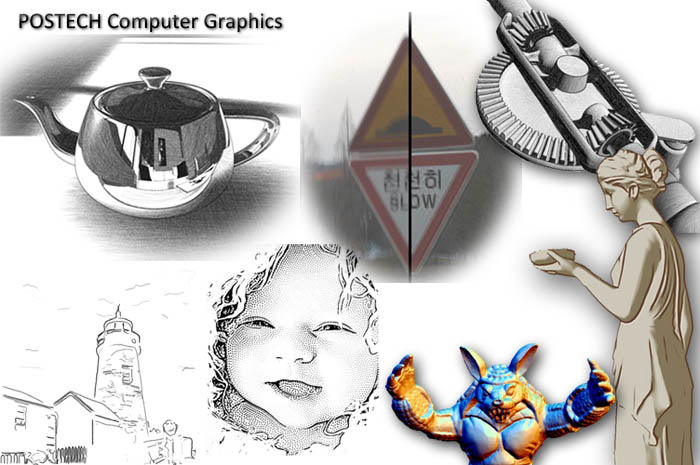
\includegraphics[width=0.5\textwidth]{intro.jpg}
%  \caption{Teaser image. (10pt)}
%  \label{fig:teaser}
%}

%% Abstract.
\begin{abstract}

요약의 제목 글꼴 크기는 (굵게, 14pt), 내용 글꼴 크기는 (10pt)입니다. 논문의 요약문은 1단 (column)으로 작성하시기 바랍니다.

\end{abstract}

%% English abstract.
%\begin{enabstract}
%
%The ``Abstract'' title should be written in (bold, 14pt) font size and contents should be written in (10pt).
%Please write abstract of the paper.
%
%\end{enabstract}

%% Keywords that describe your work.
\keywords{키워드1, 키워드2, 키워드3, 키워드4 \ldots (10pt, 주요 순서대로 핵심어를 넣는다.)}
\enkeywords{keyword1, keyword2, keyword3, keyword4 (10pt)}

%% The ``\maketitle'' command should be excuted after abstract section and keywords are written.
\maketitle

%---------------------------------------------------------------------------
% paper begins

\section{서론 (굵게, 14pt)}
\label{sec:introduction}
(논문의 내용은 10pt로 작성한다.)
온라인으로 처리되는 주요 시스템은 다음과 같다.
학회 회원 가입, 회원들의 정보 DB화, 저널투고 및 심사, 
학술대회 안내 및 학술대회 논문투고.


\section{논문 작성 요령}
\label{sec:paper_writing_technique}


\subsection{논문 페이지 수 (굵게, 12pt)}
\label{subsec:paper_page_num}

10 페이지 이내.


\subsection{용지 및 여백처리}
\label{subsec:paper_and_margin}

용지: A4, 가로쓰기. \\
여백: 위쪽 30mm, 아래쪽 20mm, 왼쪽 10mm, 오른쪽 10mm.


\subsection{글꼴 및 크기}
\label{subsec:paper_font}

한글의 글꼴은 \{serif: 바탕, sans-serif: 고딕\}을 사용하며, 
영문은 \{serif: Times New Roman, sans-serif: Helvetica\}를 사용한다. 
본문의 내용은 기본적으로 serif 글꼴을 이용하여 작성한다.
글꼴의 크기는 각각의 내용 뒤의 괄호 안에 명시된 바와 같다.

본문의 줄 간격은 한글에서는 150\%, 워드에서는 1줄로 사용한다.


\subsection{논문구성}
\label{subsec:paper_structure}

아래 순서대로 작성하며, 1$\sim$8항목은 1단 (column), 
9$\sim$11 항목은 2단으로 구성한다.

\begin{enumerate}
	\item 제목 (국문)
	\item 저자명 (국문), 발표자는 공동저자와 구분 처리한다 (예) 홍길동$^{\circ}$).
	\item 소속 (국문)
	\item 저자 e-mail address
	\item 제목 (영문)
	\item 저자명(국문), 발표자와 교신저자는 공동저자와 구분 처리한다. (예) 발표자: 홍길동$^{\circ}$, 교신저자: 홍길동$^{*}$)
	\item 소속 (영문)
	\item 요약
	\item 본문
	\begin{itemize}
		\item[-] 장 및 절에 해당되는 번호는 아라비아 숫자로 각각 1., 1.1 등과 같이 표기한다.
		\item[-] 그림의 명칭은 하단에, 표는 상단에 각각 Figure 1 및 Table 1로 표기하고 내용 또한 영문으로 작성한다.
	\end{itemize}
	\item 참고문헌
	\begin{itemize}
		\item[-] 본문 중에 참고문헌 번호를 쓰고, 그 문헌을 참고문헌란에 인용한 순서대로 기술한다.
		\item[-] 기술 순서는 아래의 예와 같이 저자, 제목, 학술지명, 권, 호, 쪽수 발행년도 순으로 작성한다.
	\end{itemize}
	\item 부록 (해당사항이 있는 경우만 작성한다.)
\end{enumerate}


\section{기타}
\label{sec:misc}

논문 작성 시 \ref{sec:paper_writing_technique}절에 명시된 요령을 지켜 주시기 바랍니다.


\section*{감사의 글}

감사의 글은 논문의 끝에 번호 없이 작성한다.

%---------------------------------------------------------------------------
% references

\bibliographystyle{IEEEtran}
\nocite{*}
\bibliography{ref}

%---------------------------------------------------------------------------
% done

\end{document}
